\chapter{Collider Phenomenology}
In this chapter, we will discuss how to connect theory and experiment. We will begin by connecting scattering amplitudes and physically observed cross sections, after which we will briefly discuss detector components of the LHC, and then move on to the question of how we establish statistical significance given experimental data from detectors.
% Scattering amplitudes and cross sections\\
\section{Detector design for hadron colliders}
Particle colliders can broadly be classified as lepton or hadron colliders. Each one has its advantages and disadvantages. Lepton colliders have cleaner signals than hadron colliders due to the lack of large QCD backgrounds. On the other hand, hadron colliders are able to reach much larger center-of-mass energies. This is because leptons, when forced along a circular path, lose large amounts of energy via synchrotron radiation. In this work, we will focus on the phenomenology of hadron colliders, both present and future.

We will first begin by describing the components of a generic detector at a hadron collider such as the LHC. At the Large Hadron Collider at CERN, the two major experiments are ATLAS (A Toroidal LHC Apparatus) and CMS (Compact Muon Solenoid). The detectors used by these experiments differ slightly in construction, but essentially probe the same physics. A cutaway view of the ATLAS detector is shown in \label{fig:ATLAS_cutaway}.

\begin{figure}[h]
  \begin{sidecaption}
    { Cutaway view of the ATLAS detector, showing the various components. Taken from \citep{Atlas2008}.}
    \centering
  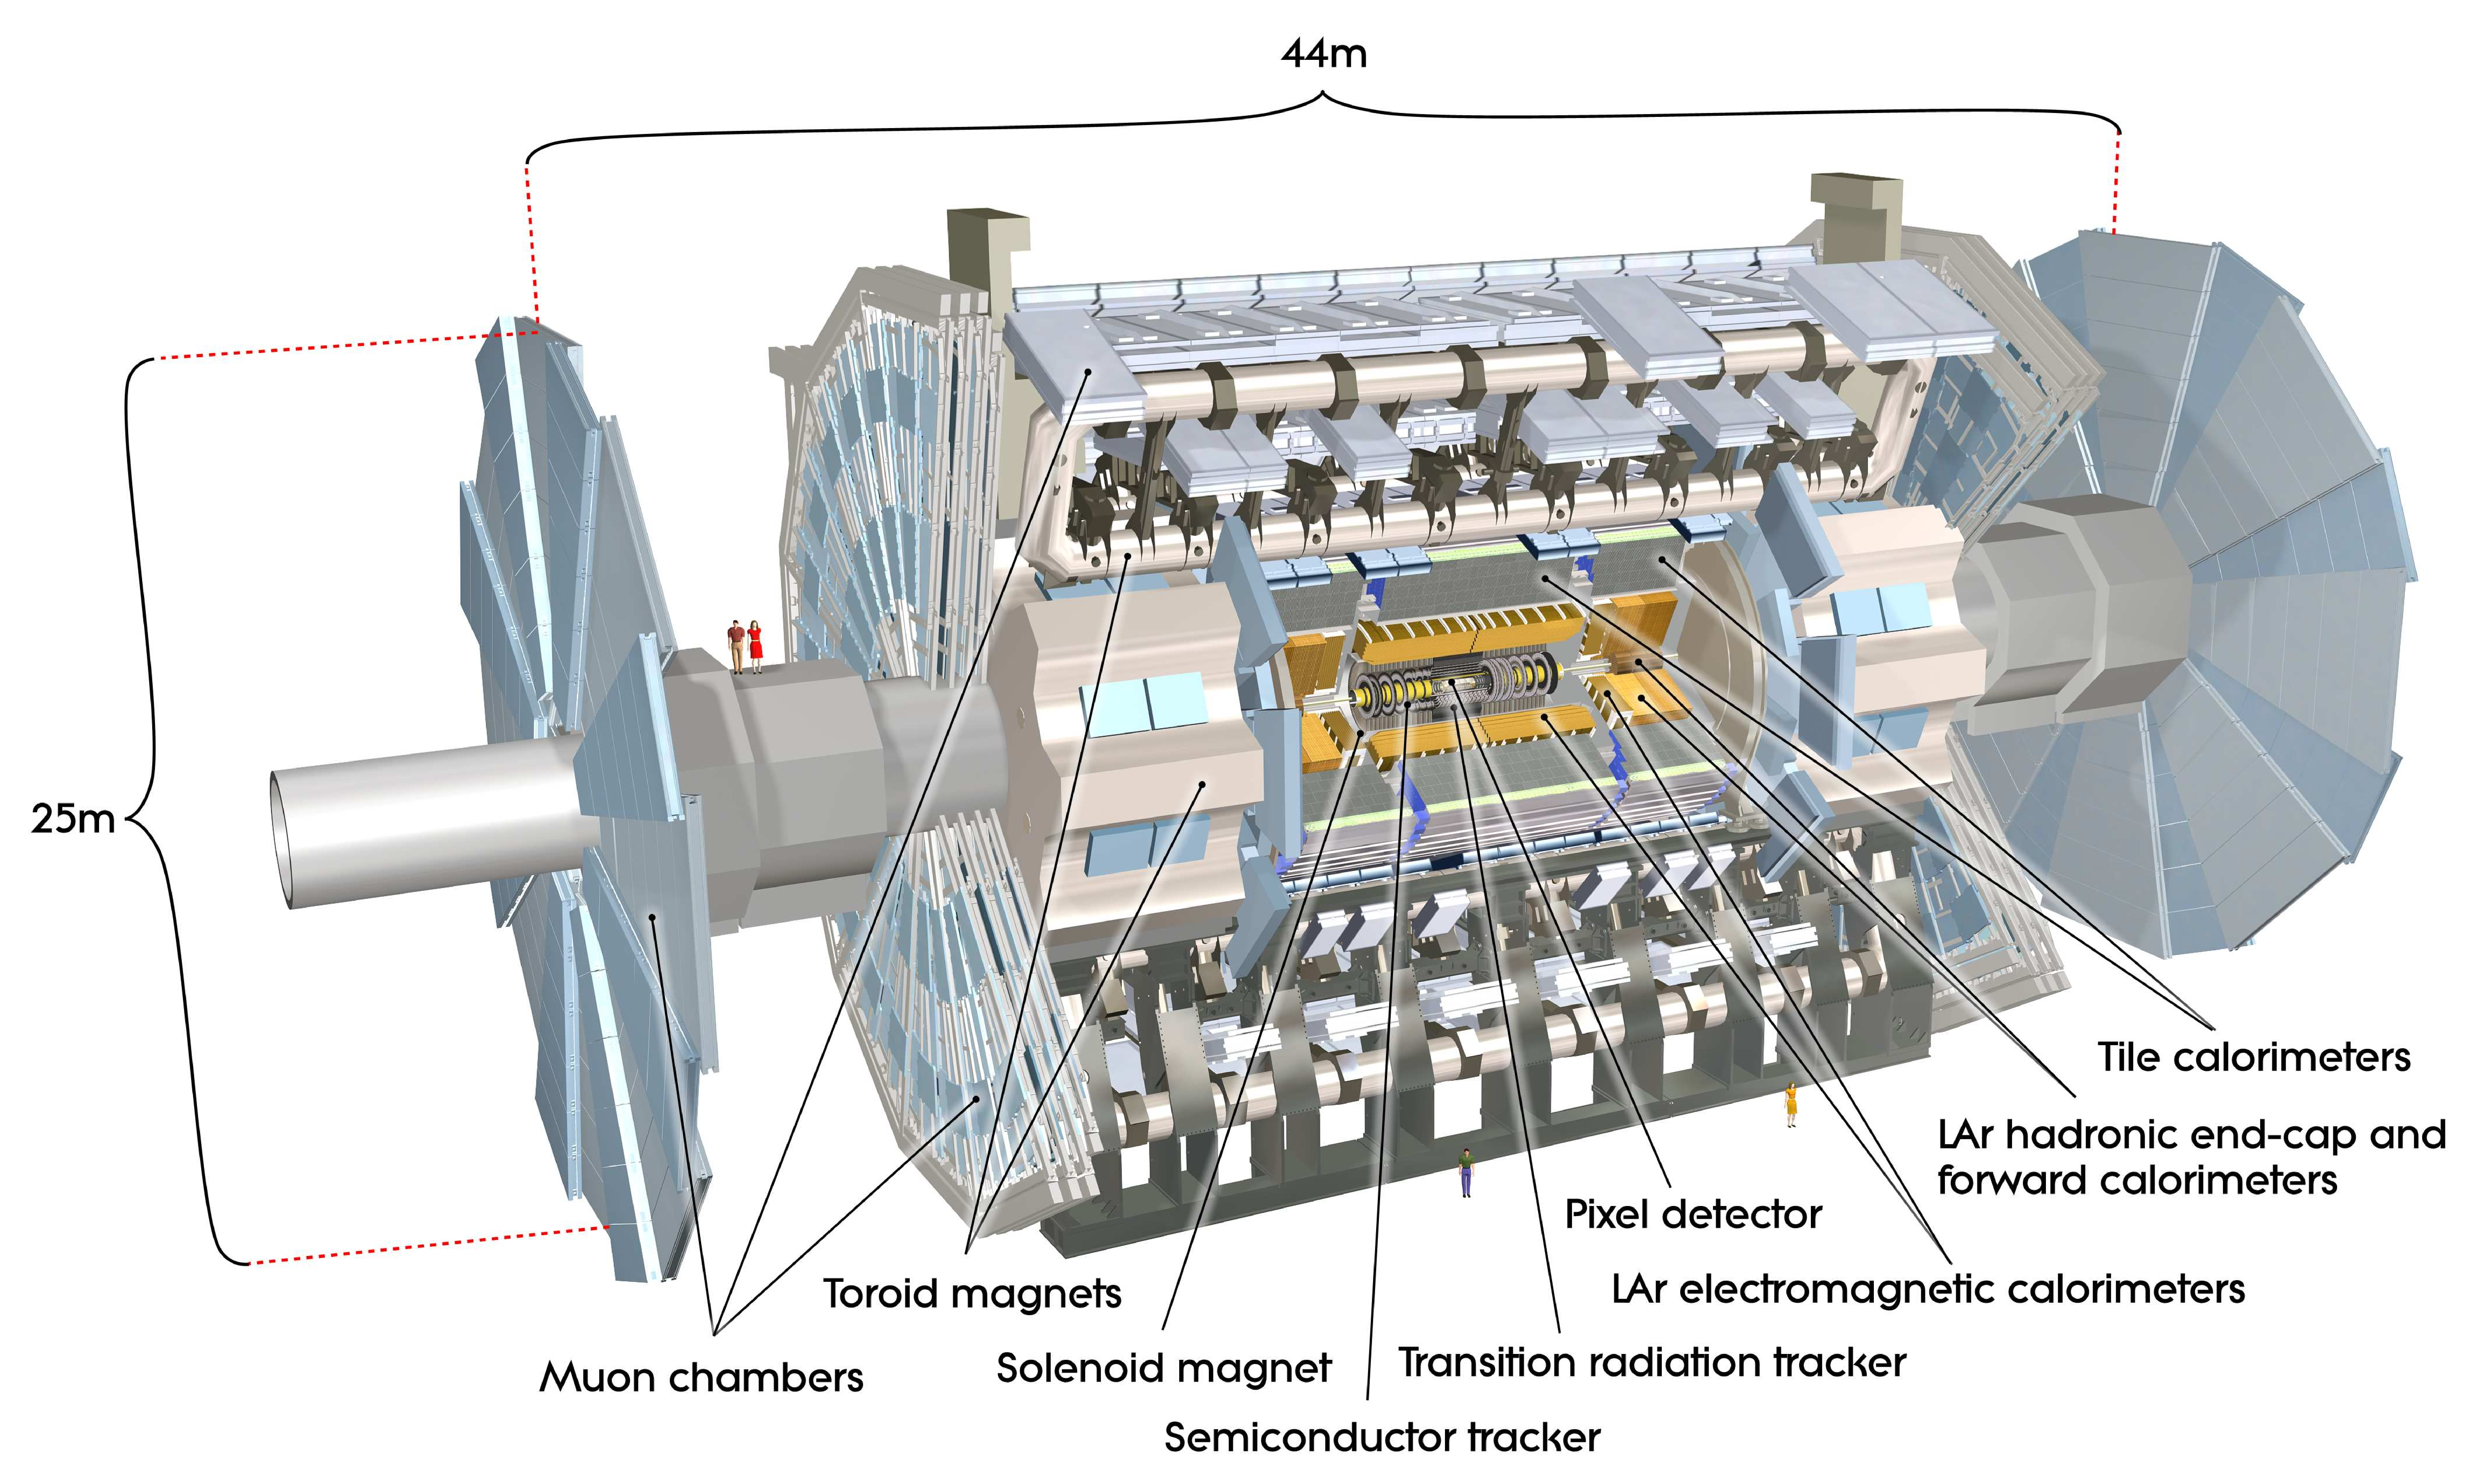
\includegraphics[trim = {2cm 5cm 2cm 2cm}, clip, width=1\textwidth]{images/atlas}
  \end{sidecaption}
  \label{fig:ATLAS_cutaway}
\end{figure}

\paragraph{Tracking chamber}
The innermost part of the detector is the tracking chamber. It consists of layers of solid-state detectors that can accurately measure the paths of charged particles that are formed in the particle collision events. The presence of a strong magnetic field bends the paths of these particles, and enables us to learn about their charge and mass.
\paragraph{Calorimeter(s)}
If a particle is energetic enough to go beyond the tracking chamber, it enters the calorimeter region. A calorimeter consists of materials dense enough to completely absorb the energy of an incident particle and stop it in its tracks. At ATLAS and CMS, the calorimeter is actually a combination of two layers that are designed to stop different particles. The electromagnetic calorimeter is designed to measure the energy of electrons and photons, while the hadronic calorimeter is designed to stop (and you might have guessed this already) hadrons. The implementation of the calorimeter depends on the detector. ATLAS has two kinds of calorimeters, one based on interleaved layers of liquid Argon and lead, and the other other based on iron and scintillating tiles. The former is used for measuring both hadronic and electromagnetic activity, while the latter specializes in hadronic calorimetry. 
\paragraph{Muon chambers} The muon is able to penetrate through the other layers.

\section{Future circular colliders}

\begin{figure}[h]
  \begin{sidecaption}
    {Schematic diagram of the FCC ring. Tunneling under Lake Geneva will be a major challenge for the construction of the ring.}
    \centering
  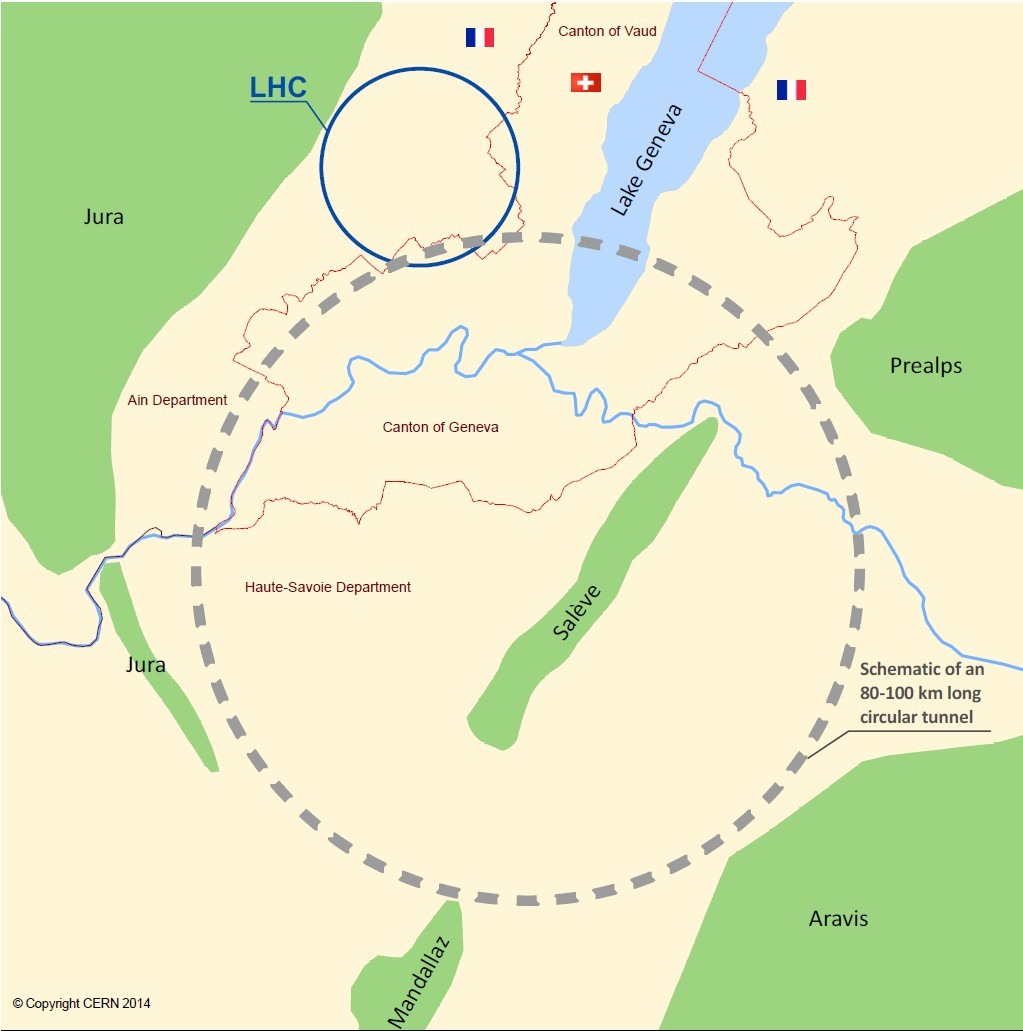
\includegraphics[width=0.9\textwidth]{images/FCC_ring_schematic}
  \end{sidecaption}
\end{figure}
\section{Anatomy of a collider analysis}
\subsection{Monte Carlo simulations}
\subsection{Showering and hadronization}
\subsection{Detector simulation and reconstruction}
\section{Statistical significance in particle physics}
